\subsection{The Implementation of Figure \ref{plot_asy}}\label{sec:App_FiniteSample}
In order to implement Figure \ref{plot_asy} from Section \ref{introductionbagging} we proceed as follows. \\
Let $Y_i \sim \mathcal{N}(0,4)$. Fix a sample $n$ from the set $\{100, 1000, 10000, 50000\}$ and denote a data set as $\mathbf{Y}=\{Y_i\}_{i=1}^n$.
The number of gridpoints for $x$ in the interval $[-5,5]$ is chosen to be $100$.
For the Bagging predictor the number of bootstrap samples is set to $B=100$.
The number of Monte Carlo iterations in order to calculate the mean squared error is also set to 100.
In every iteration step $j \in B$ at each gridpoint, we do the following:
\begin{itemize}
\item Draw a data set $\mathbf{Y_j}=\{Y_i\}_{i=1}^n$
\item Draw 100 bootstrap samples with replacement from $\mathbf{Y_j}$ and calculate for each bootstrap sample the arithmetic mean, $\bar{Y}_{n}^{*}.$ 
\item Calculate the bagged predictor according to Definition \ref{bagging}, that is $\hat{\theta}_{n;B}(x) = \frac{1}{100}\sum_{b=1}^{100}\mathbbm{1}_{[\bar{Y}_{n,b}^{*} \leq x]}.$
\item Calculate the squared error for the unbagged and the bagged predictor compared to $\theta(x)=\mathbbm{1}_{[0 \leq x]}$, that is $(\hat{\theta}_{n}(x)-\theta(x))^2$ and $(\hat{\theta}_{n;B}(x)-\theta(x))^2$, respectively.
\end{itemize}
Averaging over the respective squared errors gives the mean squared errors from the figure at one particular gridpoint.


\subsection{Illustration of the Bagging Algorithm applied to Regression Trees.}
\label{App:Ill_Bag}
Figure \ref{fig:Ill_Bag} illustrates the prediction procedure of the Bagging algorithm applied to Regression Trees. In this graphic $x$ is the covariate vector of new realizations. 
Each Tree corresponds to a bootstrapped predictor $\hat{\theta}_n(\mathbf{x})$. 
The orange paths in the trees correspond to the prediction procedure as described in Section \ref{sec:Tree_Pred}.\\
Here, + denotes the averaging over all predictions obtained by the bootstrapped predictors. The bagged prediction is denoted as $y$.

\begin{figure}[H]
\centering
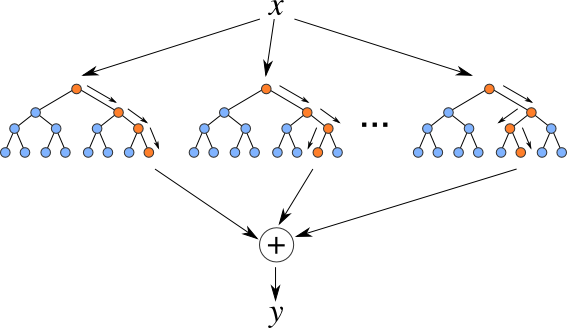
\includegraphics[scale=0.6]{Bagging/baggedtree.png}
\caption[Graphical Illustration of the Bagging algorithm applied to Regression Trees.]{Graphical Illustration of the Bagging Algorithm applied to Regression Trees. \textit{Source:} \url{http://jason-zhuo.github.io/random-forest-clustering/}.}\label{fig:Ill_Bag}
\end{figure}

